\documentclass[tikz]{standalone}
\usepackage{amsmath,amssymb}
\usepackage{tikz}
\usetikzlibrary{
	shapes,
	snakes,
	calc,
	decorations,
	decorations.markings,
	decorations.text,
	decorations.pathreplacing}
	
\begin{document}
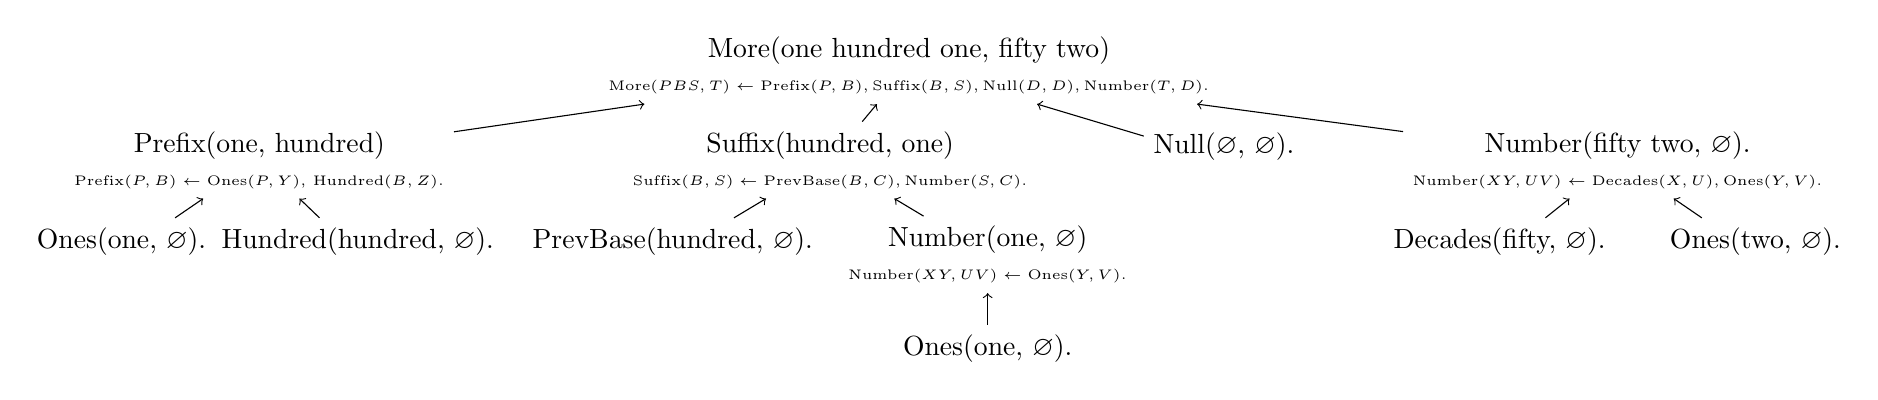
\begin{tikzpicture}[scale=1,auto,every text node part/.style={align=center}]
    % Parse Tree
  \node (M0) at (0,2.4) {More(one hundred one, fifty two)\\
    \tiny$\text{More}(PBS,T) \leftarrow \text{Prefix}(P,B), \text{Suffix}(B,S), \text{Null}(D,D), \text{Number}(T,D).$};
  \node (P1) at (-8.25,1.2) {Prefix(one, hundred)\\
    \tiny$\text{Prefix}(P,B) \leftarrow \text{Ones}(P,Y),\,\text{Hundred}(B,Z).$};
  \node (S1) at (-1,1.2) {Suffix(hundred, one)\\
    \tiny$\text{Suffix}(B,S) \leftarrow \text{PrevBase}(B,C), \text{Number}(S,C).$};
  \node (N1) at (4,1.2) {Null($\varnothing$, $\varnothing$).\\};
  \node (Nu1) at (9,1.2) {Number(fifty two, $\varnothing$).\\
    \tiny$\text{Number}(XY,UV) \leftarrow \text{Decades}(X,U), \text{Ones}(Y,V).$};
  \node (O2) at (-10,0) {Ones(one, $\varnothing$).\\};
  \node (H2) at (-7,0) {Hundred(hundred, $\varnothing$).\\};
  \node (PB2) at (-3,0) {PrevBase(hundred, $\varnothing$).\\};
  \node (N2) at (1,0) {Number(one, $\varnothing$)\\
    \tiny$\text{Number}(XY,UV) \leftarrow \text{Ones}(Y,V).$};
  \node (D2) at (7.5,0) {Decades(fifty, $\varnothing$).\\};
  \node (On3) at (10.75,0) {Ones(two, $\varnothing$).\\};
  \node (O3) at (1,-1.2) {Ones(one, $\varnothing$).};

  \draw [<-] (M0)     to (P1);
  \draw [<-] (M0)     to (S1);
  \draw [<-] (M0)     to (N1);
  \draw [<-] (M0)     to (Nu1);
  \draw [<-] (P1)     to (O2);
  \draw [<-] (P1)     to (H2);
  \draw [<-] (S1)     to (PB2);
  \draw [<-] (S1)     to (N2);
  \draw [<-] (N2)     to (O3);
  \draw [<-] (Nu1)    to (D2);
  \draw [<-] (Nu1)    to (On3);

\end{tikzpicture}
\end{document}
